\section{Программная реализация}
\label{sec:Chapter3} \index{Chapter3}
Требуется реализовать блочное разбиение области между процессами, поскольку в этом случае предполагается меньше межпроцессорных коммуникаций, по сравнению с ленточным.

\captionsetup[subfloat]{labelformat=empty}
\begin{figure}[H]
    \centering
    \subfloat[Ленточное разбиение 3d]{%
        \raisebox{-0.5\height}{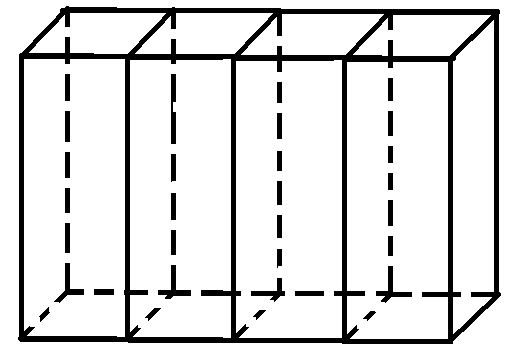
\includegraphics[width=.49\linewidth]{./images/0.png}}%
    }
    \hfill
    \subfloat[Блочное разбиение 3d]{%
        \raisebox{-0.5\height}{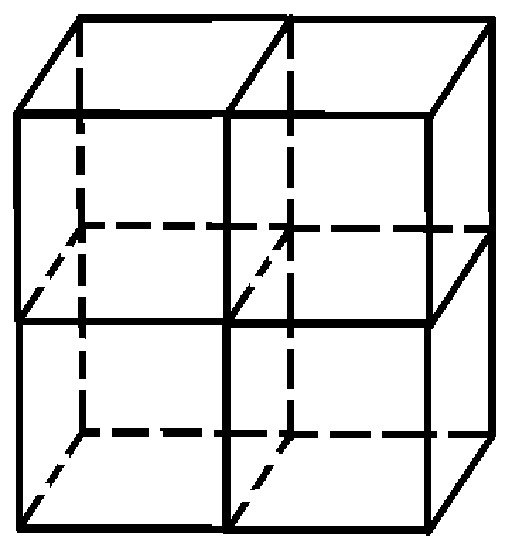
\includegraphics[width=.49\linewidth]{./images/1.png}}%
    }
    \caption{Виды разбиений 3d}
    \label{fig:1}
\end{figure}

Число областей, на которое необходимо произвести разбиение может быть произвольным, как четным, так и нечетным. 

На рисунке \ref{fig:1} изображен схематично двумерный ленточный и блочный вариант разбиения квадратной области на 8 частей. 

В случае ленточного разбиения получаем \(S_{strip}=8L\) межпроцессорных коммуникаций.
В блочном случае \(S_{block}=8(L/2)+4(L/4)=5L\) коммуникаций, то есть в 1.6 раз меньше.
С ростом числа разбиений (и процессов, соответственно) это число будет только увеличиваться.
Данные рассуждения можно обобщить и на трехмерный случай.

\begin{figure}[H]
    \centering
    \subfloat[Ленточное разбиение]{%
        \raisebox{-0.5\height}{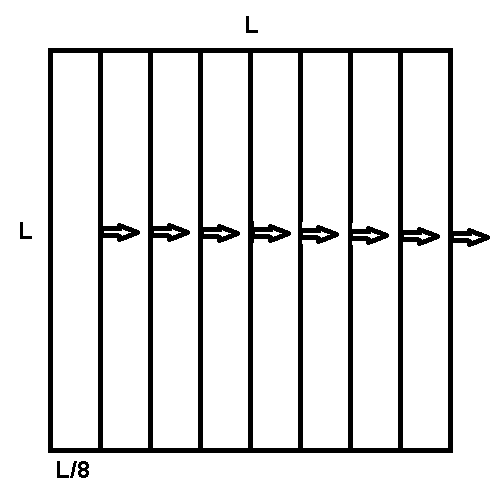
\includegraphics[width=.49\linewidth]{./images/2.png}}%
    }
    \hfill
    \subfloat[Блочное разбиение]{%
        \raisebox{-0.5\height}{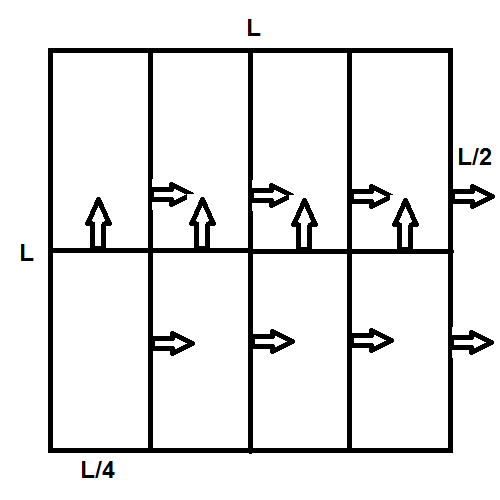
\includegraphics[width=.49\linewidth]{./images/3.png}}%
    }
    \caption{Виды разбиений}
    \label{fig:2}
\end{figure}
Таким образом, алгоритм решения задачи, выглядит следующим образом:
\begin{enumerate}
    \item Исходя из варианта, расчитывается точное аналитическое решение \(u_{analytical}\) в узлах сетки.
    \item Проводим разбиение области \(\Omega\) между процессами.
    \item Фиксируем временной слой (начиная с \(0\)). 
    \item Используя формулы (\ref{equation:10}) и (\ref{equation:12}). находим значения \(u^0\) и \(u^1\).
    \item Пользуясь найденными \(u^0\) и \(u^1\) и разностным представлением уравнения (\ref{equation:1}), находим значения \(u\) в локальной области разбиения. 
    \item Передаем посчитанные граничные значения блокам-соседям.
    \item Повторяем шаги 5--6 для внутренних блоков.
    \item Определяем максимальную погрешность на сетке между посчитанным и аналитическим решением.
    \item Переходим на следующий слой по времени и повторяем шаги 2--9.
\end{enumerate}


\lstset{
backgroundcolor=\color{gray!10},
frame=single,
basicstyle=\ttfamily\small,
breaklines=true,
columns=fullflexible
}
Реализация данного алгоритма была написана на языке C++ и выложена на GitHub (https://github.com/Marilius/edu-cmc-skmodel26).
Для компиляции и запуска использовались подобные команды (версия с OpenMP):
\begin{lstlisting}[language=Bash, caption=Пример запуска с OpenMP]
g++ -O2 -fopenmp -std=c++11 src/main.cpp -o solver.out
mpisubmit.pl -t 8 solver.out --stdout std.out --stderr std.err \
-- 128 20 1. 1. 1. 0.01
\end{lstlisting}

% TODO
% Lx = Ly = Lz = 1, Lx =
% Ly = Lz = 